\documentclass[12pt]{article}
\usepackage{amsmath,amssymb,bookmark,graphicx,parskip,custom}
\usepackage[margin=.8in]{geometry}
\allowdisplaybreaks
\hypersetup{colorlinks,
    citecolor=black,
    filecolor=black,
    linkcolor=black,
    urlcolor=black
}
\setcounter{secnumdepth}{5}

\begin{document}

\title{SCI 238 --- Introduction to Astronomy}
\author{Kevin James, Nik Klassen}
\date{\vspace{-2ex}Winter 2015}
\maketitle\HRule

\tableofcontents
\newpage

\section{Chapter 1 -- Our Place in the Universe}
\subsection{Overview}
A naive look at the sky, which seems to rotate around us, implies we live in a {\bf geocentric} Universe, ie. that everything orbits around the Earth. We know now that this is untrue, but the path to this knowledge was a long one.

We can refer to our place in the Universe as our {\bf cosmic address}, this is our {\bf solar system}; which consists of the Sun and all objects that orbit it including rocky {\bf asteroids} and icy {\bf comets}. Our solar system, and all the stars we can see, make up a small portion of the {\bf Milky Way} galaxy.

A {\bf galaxy} is an island of stars in space containing anywhere between a few hundred million to trillions of stars. The Milky Way is a relatively large one, with 100 billion stars. We are located about halfway from the center of the Milky Way (the {\bf galactic center}) to the edge of the {\bf galactic disk}.

In summary: the Earth is a planet in the solar system, which is a collection of objects orbiting a star, which is in the milky way galaxy, which is a part of the {\bf local group} of galaxies, which is part of the {\bf local supercluster} of groups, which is somewhere in the {\bf Universe}.

The local group contains about 40 galaxies, and is one of what we call {\bf galactic clusters} -- groups of galaxies with more than a few members. Superclusters are essentially clusters of galactic clusters, as the Universe seems to be arranged ingiant chains and sheets with large divides between them. The local group is on the edge of the local supercluster.

\subsection{The Big Bang and the Expanding Universe}
We have observed that the Universe seems to be \emph{expanding}, that is, the distance between galaxies is increasing. By extrapolating backwards, we imagine that all matter must ahve existed at the same point in the past and exploded outward in a {\bf Big Bang}. Based on the rate of expansion, we believe this happened approximately 14 billion years ago.

Note that though the distance between galaxies is increasing, the distances between objects within galaxies is \emph{not}.

Most galaxies, including our own, formed within a few billion years of the Big Bang.

\subsection{The Birth of Stars}
A star is {\bf born} when gravity compresses the material in a cloud of gas and dust until it is dense and hot enough to generate energy through {\bf nuclear fusion}. The star lives so long as it has useable material to fuel its fusion and dies once it runs out.

A star {\bf dies} by blowing much of its remaining content back into space in a {\bf supernova}. This matter eventually becomes new stars and planets.

\subsection{Modelling the Universe}
\subsubsection{Distance}
We can imagine our solar system shrunk down to a manageable size. On the {\bf Voyage} scale (a model solar system in Washington, D.C. where sizes are one billionth of the actual size), the Sun is roughly the size of a grapefruit, Jupiter the size of a marble, Earth the size of a pinhead. Obviously the Sun is far larger than any planet, in fact, it has more than 1000 times as much mass as all the planets in our system combined. Note that the planets also vary in size to a large extent: the ``permanent'' storm on Jupiter known as the {\bf Giant Red Spot} is larger than the Earth.

We can also use this model to describe the distances between objects. On the same scale, the Earth is 15m from the Sun and the distance from the Sun to pluto is 600m. To have enough space for the orbit of each object in the system, we would need a grid of 300 football fields centered around the Sun.

The closest star (Alpha Centauri) is incredibly far away, on this scale it would be the difference between Washington, D.C. and California.

If we reduce this scale by another factor of one billion, we can start thinking about the size of the galaxy. On this scale, each light year is roughly a millimeter and the Milky Way is about the size of a football field. The distance between our star system and Alpha Centauri is smaller than the width of our pinky.

\subsubsection{Time}
We can also model the time between events by creating a {\bf cosmic calendar}. If we set the Big Bang as January $1^{st}$ and the present day as Decembre $31^{st}$, we can place each major event on specific days. By the age of the universe, each month represents just over a billion years.

On this scale, the Milky Way was formed sometime in February. Our solar system, though was, only formed in September -- life on Earth flourished by the end of that month. Recognizeable animals only appeared in mid-December. Dinosaurs first appeared the day after Christmas and died off yesterday. Around 9PM today, early hominids began to walk upright.

The entire history of human civilization, then, occurred in the last half-minute of January $31^{st}$.The Egyptians built the pyramids in 11 seconds, Galileo proved the Earth orbited the Sun one second ago, and the average college student was born 0.05 seconds ago.

\subsection{Motion of the Universe}
The Earth has a daily rotation (its {\bf spin}) and a yearly {\bf orbit} (or {\bf revolution}) around the Sun.

The Earth rotates each day around its {\bf axis}, the imaginary line from the North to the South pole. It rotates from West to East -- counter-clockwise when viewed from above the North pole. The speed is substantial; anywhere other than near the axes, an object whirls around the Earth at a speed greater than 1000km/h.

The Earth's average orbital distance is one {\bf Astronomical Unit} (AU), which is approximately 150 million kilometers. At times, we race around the Sun in excess of one hundred thousand kilometers per hour.

Earth's orbital path defines the {\bf eliptic plane}, and its axis is tilted by 23.5 degrees from a line perpendicular to this plane. The {\bf axis tilt} happens to align our north pole with Polaris, the North Star.

Note that the Earth orbits the Sun in the same direction as it spins around its axis since it was formed from a spinning disk and both of these rotations are a remnant of this.

We also move relative to nearby stars at a rate of $70,000$ kilometers per hour. We rotate around the Milky Way's galactic center once every 230 million years, which implies speeds of (on average) $800,000$ kilometers per hour.

\subsection{Dark Matter and Dark Energy}
Since stars at different distance from the galactic center orbit at different speeds, we can learn how mass is distributed in the galaxy by measuring the differing speeds. Studies show that the mass of the stars in the galactic disk form only a small percentage of the total mass of the galaxy. Most of the galactic mass, then, seems to be located outside of the visible disk in the galaxy's {\bf halo}. We call this mass {\bf dark matter}, since we have not observed light being emitted from it. Similarly, we find that the bulk of the energy in the universe is {\bf dark energy}. This seems to be the case in all observable galaxies.

\subsection{Relative Galactic Movements}
Within the local group, some galaxies move toward us and some move away. Outside of the local group, though, this changes; virtually every galaxy outside of the local group seems to be racing away from us at a speed proportional to its distance from us. This is the basis of our theory that of an {\bf expanding universe}: that the space between galaxies is increasing.

Note that we observe this motion by measuring {\bf Doppler shifts}, as detecting any difference in celestial position within our lifetimes is impossible.

\section{Chapter 2 -- Discovering the Universe}
\subsection{The Motion of the Stars}
Stars appear to move across the sky from east to west. This is not, as the ancients believed, because everything revolves around the Earth, but because the Earth is rotating. This rotation is not perfect though, because the Earth is tilted.

Some stars (those near the celestial north pole) do not rise or set; they remain above the horizon and make daily counter-clockwise circles around the pole. These stars are called {\bf circumpolar} stars. Other stars (those near the celestial south pole) never rise at all. All other stars appear to rise and set each day.

\subsection{Constellations}
Although we have a colloquial definition of constellations, astronomers more precisely declare {\bf constellations} to be regions of the sky with well-defined borders. The patterns of stars which ``form'' constellations simply help us to locate them.

There are 88 official constellations which cover the night sky, as determined by a 1928 summit including members of the International Astronomical Union. Every part of the sky is located within one of these constellations.

Though the stars are very far away, the ancient Greeks believed they were all ``painted'' on a {\bf celestial sphere} centered around the Earth. We use this today to help us map out space:
\begin{itemize}
\item the {\bf north celestial pole} is directly above the north pole, and
\item the {\bf south celestial pole} is directly above the south pole, and
\item the {\bf celestial equator} mirrors the real equator, and
\item the {\bf ecliptic} is the path the Sun takes as it appears to circle around the celestial sphere yearly. It crosses the celestial equator at a 23.5 degree angle
\end{itemize}

The {\bf Milky Way} traces a complete circle around the celestial sphere, moving through many constellations. It is almost, but not quite, repesentative of the Milky Way \emph{Galaxy}: it traces our galaxy's disk of stars as it appears from our location in the outskirts of the galaxy. The Milky Way appears somewhat wider as we look through Sagittarius since this is the direction of the galactic center.

Note that when looking above you at the {\bf local sky}, you can (obviously) only see one hemisphere of the celestial sphere at a time. We define the Earth-sky boundary as the {\bf horizon}, the point directly overhead as the {\bf zenith}, and an imaginary semi-circle passing along the sphere from due north to due south through the zenith as the {\bf meridian}.

We can locate any object by its direction along the horizon and its altitude above the horizon. We also sometimes use the {\bf azimuth} -- the angular distance clockwise from due north.

We can define the {\bf angular size} of an object as the angle it appears to span within our field of view. Since this depends on distance, it does not give us a clear idea of an object's true size; for example, the angular size of both the Sun and the Moon is half a degree despite the Sun being about 400 times larger (since the Sun is 400 times farther away).

The {\bf angular distance} between two objects is the number of degrees which appears to separate them. The distance between the pointer stars in the big dipper is roughly 5 degrees. We further divide each degree into 60 {\bf arcminutes} -- and then each of those into 60 {\bf arcseconds} -- for precision.

\subsubsection{Variance}
Constellations vary with both our north-south location on Earth as well as the time of year.

{\bf Latitude} affects the constellations by changing the locations of the horizon and zenith of our local sky. In effect, by moving to the north or south we can change which portion of the celestial sphere is visible. We can also use this effect to prove that \emph{the altitude of the celestial pole in your sky is equal to your latitude}.

The constellations vary over the course of the year due to Earth's changing position around the Sun. As we orbit, the Sun appears to move across the eliptic such that different stars are behind it at different times of the year. The constellations along this eliptic make up the {\bf zodiac}, the thirteen most widely known constellations (traditionally, there are twelve zodiacs; however, Ophiuchus is also present in the eliptic).

\subsection{Seasons}
The seasons are caused by the tilt of the Earth's axis. In effect, the axis remains pointing at a specific direction in space at all times. This, of course, means it is pointing at different points relative to the Sun throughout the year. The Northern Hemisphere is tipped toward the sun in their summer (June), and vice-versa. This causes the Sun's rays to hit the ``closer'' hemisphere for a longer time each day during their summer, as well as concentrating its rays, thus making it warmer.

Note that the common assumption is the summer occurs when the Earth is closer to the Sun than it is during winter. This is incorrect; in fact, the orbital distance between the Earth and the Sun \emph{does} vary, but only by approximately $3\%$. This difference does not cause noticeable temperature changes.

\subsubsection{Solstices}
We mark the special celestial events each year as the {\bf solstices} and {\bf equinoxes}:
\begin{itemize}
\item the {\bf summer (June) solstice} occurs around June $21^{st}$. It is the moment in which the Norther Hemisphere is tipped most directly toward the Sun.
\item the {\bf winter solstice} occurs around December $21^{st}$ and is precisely the opposite of the summer solstice.
\item the {\bf spring equinox} occurs around March $21^{st}$ and is the moment at which the Northern Hemisphere switchees from being slightly tipped away from the Sun to slightly toward the Sun.
\item the {\bf fall equinox} occurs around September $22^{nd}$ and is precisely the opposite of the spring equinox.
\end{itemize}

The exact dates vary each year by no more than a few days in either direction. In fact, our leap year system is designed precisely to ensure this is true.

The equinoxes are the only days of the year in which the Sun rises and sets exactly due East and West, as well as being the only days in which an equal amount of sunlight falls on both Hemispheres. The Sun rises and sets farther to the North on the Summer solstice side of the equinoxes, and farther South on the Winter solstice side.

We usually consider the solstices and equinoxes as the first day of the new season, despite the summer solstice, for example, being the longest day of the year -- ie. the midpoint of summer? This is generally due to weather patterns; the solstices and equinoxes match the beginning of the new season's weather patterns. We also find the it takes some time to match the temperature of the Earth to the Sun's location, thus making us feel a lag behind what the Sun implies our temperature should be.

Note that te solstices are named opposite to the seasons in the Southern Hemisphere. For the equator, we find that the rainy seasons occur at the equinoxes and the dry seasons occur at the solstices.

\subsection{Precession}
{\bf Precession} is a slow wobble of the Earth's tilt which affects our orientation in space. Each precession cycle takes approximately $26,000$ years and slowly changes where our poles point to in space. Today, our axis points toward Polaris, which we call the North Star. In approximately $13,000$ years, Vega will be in this location (ie. a bright star very near the pole's zenith). Most of the time, there is no North Star.

Precession, though, does not change the amount of tilt we have relative to the eliptic; we always have a 23.5 degree tilt, and so our seasons are not affected by precession.

Precession is caused by the effect of gravity on a rotating object which is not a perfect sphere. For the Earth, precession is caused by the competing effects of gravity from the Sun and the Moon attempting to ``straighten out'' our bulging equator.

\subsection{The Moon}
The Moon orbits the Earth once every $27.\bar{3}$ days. We can see that the Moon appears to move across the sky at half a degree (it's angular size) per hour. As it moves across the sky, its appearance and rising / setting times change according to its {\bf lunar phase}, which is based on its position relative to the Sun as it orbits the Earth.

The change of appearance is based on the direction the Sun casts its light from. When the Moon, Earth, and Sun form a right-angle, the Sun casts its light in such a way that only half of the Moon is illuminated from the Earth's perspective. The lunar cycle takes $29.5$ days to complete.

The Moon appears to fill in illumination starting from the right, then lose illumination from the same direction. We refer to completely dark Moons as {\bf New Moons} and completely illuminated ones as {\bf Full Moons}. {\bf Crescent Moons} and {\bf Gibbous Moons} (barely illuminated and almost fully illuminated, respectively) are refered to as {\bf waxing} or {\bf waning} depending on whether it is between a New Moon and a Full Moon or vice-versa. Half-illuminated Moons are referred to as the {\bf First and Third Quarter Moons}.

\begin{figure}[ht]
\centering
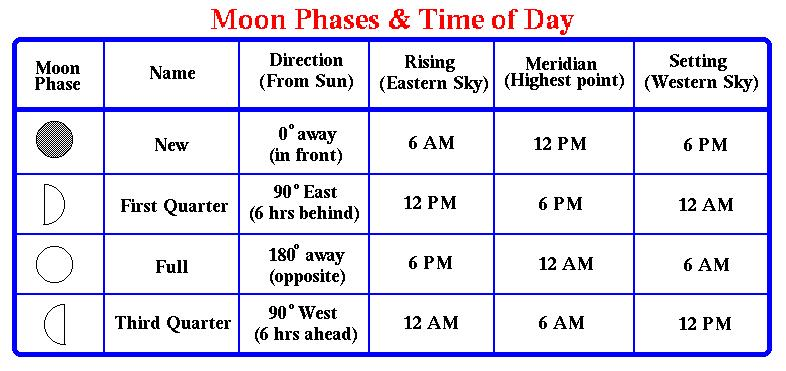
\includegraphics[width=0.7\textwidth]{moon_phases.jpg}
\end{figure}

\subsubsection{Eclipses}
Eclipses occur when the Sun, Moon, and Earth are aligned. A {\bf lunar eclipse} occurs when the Earth lies between the other two, such that the Earth's shadow falls on and blacks out the Moon. A {\bf solar eclipse} occurs when the Moon lies between the Sun and the Earth, so that the Moon block's our view of the Sun (ie. its shadow falls on us).

Since the Moon's orbit is slightly (5 degrees) inclined, eclipses do not happen each month. Eclipses, then, only occur when the Moon passes through the ecliptic; the two locations in which it does are referred to as the {\bf nodes} of its orbit. These times are called {\bf eclipse seasons}, and occur twice per year.

A lunar eclipse occurs when a full moon occurs near a node, a solar eclipse occurs when a new moon occurs near a node.

Since the Moon's shadow has both an {\bf umbra} -- the central area which completely blocks sunlight -- and a {\bf penumbra} -- which only partially blocks sunlight -- these eclipse can look extremely different. If the three objects line up perfectly, we can have a {\bf total lunar eclipse}, in which the Moon is completely blocked during the period of {\bf totality}. More likely is a {\bf partial eclipse}, which only hides a portion of the Moon. Finally, we have {\bf penumbral lunar eclipses}, which shade the Moon but do not completely blot it out.

During totality, the Moon is completely dark for typically less than an hour, save for the red ring around it formed because Earth's atmosphere bends some of the Sun's light toward the Moon (and, to a far lesser extent, due to {\bf gravitational lensing}).

Similarly, we have total and partial solar eclipses based on whether you are within the Moon's umbra or penumbra. When the Moon is too far away for its umbra to even reach the Earth, we see an {\bf annular eclipse}: a ring of sunlight surrounding the Moon when we are directly behind the umbra; otherwise, we see a partial eclipse.

Since the umbra moves across the Earth at a speed of $1,700$ km/h, an eclipse can last no more than a few minutes for any given location on Earth.

The location of the nodes in the Moon's orbit slowly change over time. This gives us an eclipse cycle of 18 years 11.3 days; we call this the {\bf Saros Cycle}. Of course, this only tells us when eclipses will occur, not where they will be visible from on Earth or whether they will be total or partial.

\subsection{Planets}
We can see five planets with the naked eye: Mercury, Venus, Mars, Jupiter, and Saturn. Mercury is rarely visiable, and only near sunrise or sunset. Venus can often be seen shining brightly in the evening (in the West) or before dawn (in the East). Jupiter, when visible, is the brightest star at night. Mars is often recognizeable by its red hue. Saturn has no distinguishing features, but can be identified with star charts.

Planets have different paths of motion that do stars, which is why the word for planet in Greek means ``wandering star''. The planets usually move Eastward through constellations, but sometimes go through periods of {\bf apparent retrograde motion} for anywhere between a few weeks and a few months. This retrograde motion occurs when the Earth ``passes'' the other planet, ie. when their orbits are in line with the Sun.

{\bf Stellar parallax} is the phenomenon of stars appearing to move at different rates given different angles; given the extremely great distances between us and the stars, this is not detectable by the human eye -- though it can be detected by telescopes.

\section{Chapter 6 -- Formation of Planetary Solar Systems}
\subsection{Overview}
This chapter is about the nature of our solar system and current scientific ideas about its birth. We will also examine characteristics about our solar system that are key clues about how it formed. Finally it will talk about how astronomers have discovered other planets around other stars and how those planetary systems are helping us understand our own.

\subsection{Clues to the formation of the Solar System}
The Solar System's layout and composition offer 4 clues as to how it was born.
\begin{enumerate}
\item {\bf Large bodies in the solar system have orderly motions}.
\begin{itemize}
\item All planets have nearly circular orbits going in the same direction in nearly the same plane.
\item  All planets {\bf orbit} the Sun in the same direction: {\bf counterclockwise} as viewed from high above Earth’s North Pole.
\item Most planets rotate in the same direction in which they orbit, with fairly small axis tilts. The Sun also rotates in this direction.
\item Most of the solar system’s large moons exhibit similar properties in their orbits around their planets, such as orbiting in their plane
\end{itemize}
\item {\bf Planets fall into two major categories}
\begin{enumerate}
\item {\bf Terrestrial planets}
\begin{itemize}
\item Small in mass and size
\item Close to the sun
\item Made of metal and rock
\item Few moons and no rings
\end{itemize}
\item {\bf Jovian planets}
\begin{itemize}
\item Large in mass and size
\item Far from the Sun
\item Made from H, He and hydrogen compounds
\item rings and many moons
\end{itemize}
\end{enumerate}
\item {\bf Swarms of asteroids and comets populate the solar system}. Vast numbers of rocky asteroids and icy comets are found throughout the solar system, but are concentrated in 3 distinct regions
\begin{itemize}
\item Most {\bf asteroids} orbit in the {\bf asteroid belt} between Mars and Jupiter
\item Many {\bf comets} are found in the {\bf Kuiper Belt} beyond Neptune's orbit
\item Even more {\bf comets} orbit the sun in the distant spherical region called the {\bf Oort Cloud} and only a rare few ever plunge into the inner solar system. May contain a trillion comets.
\end{itemize}
\item {\bf Several notable exceptions to these trends stand out}
\begin{itemize}
\item {\bf Uranus's odd tilt} Uranus rotates nearly on its side compared to its orbit and its rings and major moons share this sideways orientation.
\item {\bf Earth's relatively large moon} Our moon is much larger in size than most other moons in comparison to their planets
\item {Venus' backwards rotation}
\end{itemize}
\end{enumerate}

\subsection{The Sun}
The {\bf sun contains more than 99.8\% of the solar systems total mass}. (1000 times more massive than the rest of the solar system combined). The surface is a sea of rolling hot (5800K) Hydrogen and Helium gas. The sun is gaseous throughout and temperture and pressure both increase with depth. In addition, charged particles moving outward ({\bf Solar wind}) help shape planetary magnetic fields and can influence planetary atmospheres.

\subsection{Mercury}
A desolate, cratered world with no active volcanoes, no wind, no rain, and no life. It is a world of both {\bf hot and cold extremes}. The combination of rotation and orbit gives Mercury days and nights that last about 3 Earth months each. Mercury’s {\bf surface is heavily cratered} But it also shows evidence of past geological activity, such as plains created
by ancient lava flows and tall, steep cliffs that run hundreds of kilometers in length. Mercury’s {\bf high density} indicates that it has a very large iron core.

\subsection{Venus}
Venus is nearly identical in size to Earth. It {\bf rotates on its axis very slowly and in the opposite direction of Earth}, so days and nights are very long. An {\bf extreme greenhouse effect} bakes Venus’s surface to an incredible 470°C. Day and night. Venus has {\bf mountains, valleys, and craters, and shows many signs of past or present volcanic activity}. But Venus also has geological features unlike any on Earth, and we see no evidence of Earth-like plate tectonics.

\subsection{Earth}
Only planet in our solar system with oxygen to breathe, ozone to shield the surface from deadly solar radiation, and abundant surface water to nurture life. Temperatures are pleasant because Earth’s atmosphere contains just enough carbon dioxide and water vapor to maintain a moderate greenhouse effect.

\subsection{Mars}
Mars has ancient volcanoes. The presence of dried-up riverbeds, rock-strewn floodplains, and minerals that form in water offers clear evidence that Mars had at least some warm and wet periods in the past. Major flows of liquid water probably ceased at least 3 billion years ago. More than a dozen spacecraft have flown past, orbited, or landed on Mars.

\subsection{Jupiter}
Most famous feature: long-lived storm called the Great Pluto. {\bf Made primarily of hydrogen and helium and has no solid surface}. Increasing gas pressure would crush us long before we ever reached its core. Jupiter reigns over dozens of moons and a thin set of rings (too faint to be seen in most photographs).

\subsection{Saturn}
Saturn is made mostly of hydrogen and helium and has no solid surface. The rings may look solid from a distance, but in reality they are made of countless small particles, each of which orbits Saturn. Titan, the only moon in the solar system with a thick atmosphere. Saturn and its moons are so far from the Sun that Titan’s surface temperature is a
frigid -180°C.

\subsection{Uranus}
It is made largely of hydrogen, helium, and hydrogen compounds such as water (H 2 O), ammonia (NH3), and methane (CH4). Uranus lacks a solid surface. The entire Uranus system—planet, rings, and moon orbits—is tipped on its side compared to the rest of the planets and it gives Uranus the most extreme seasonal variations of any planet in our solar system.

\subsection {Neptune}
Neptune looks nearly like a twin of Uranus, although it is more strikingly blue. Smaller than Uranus but more massive due to higher density (even though they have similar composition. Triton is the only large moon in the solar system that orbits its planet “backward”—that is, in a direction opposite to the direction in which Neptune rotates. This backward orbit makes it a near certainty that Triton once orbited the Sun independently before somehow being captured into Neptune’s orbit.

\subsection {Pluto (and other dwarf planets)}
Pluto is much smaller and less massive than any of the other planets, and its orbit is much more eccentric and inclined to the ecliptic plane. Its composition of ice and rock is also quite different from that of any of those planets, although it is virtually identical to that of many known comets. Pluto is not even the largest of Kuiper belt objects, Eris, is slightly larger than Pluto.

\subsection{Where did the solar system come from?}
The {\bf nebular theory} begins with the idea that our solar system was born from a cloud of gas, called the solar nebula, that collapsed under its own gravity. As the solar nebula shrank in size, three important processes altered its density, temperature, and shape, changing it from a large, diffuse (spread-out) cloud to a much smaller spinning disk: {\bf heating, spinning, flattening}. As it collapsed, it heated up, spun faster and flattened into a disk.

\subsubsection{The Formation of the planets}
In the center of the collapsing solar nebula, gravity drew together enough material to form the Sun. Because hydrogen and helium gas made up 98\% of the solar nebula’s mass and did not condense, the vast majority of the nebula remained gaseous at all times. However, other materials could condense wherever the temperature allowed.

The solid metal and rock in the inner solar system ultimately grew into the terrestrial planets we see today, but these planets ended up relatively small in size because rock and metal made up such a small amount of the material in the solar nebula. {\bf Accretion} The process in which small ``seeds'' grow into planets.

The leading model for jovian planet formation holds that these planets formed as gravity drew gas around ice-rich ``boulders'' much more massive than Earth. Their large masses had gravity strong enough to capture some of the hydrogen and
helium gas that made up the vast majority of the surrounding solar nebula. Ultimately, the jovian planets accreted so
much gas that they bore little resemblance to the icy seeds from which
they started.

The young Sun had a strong solar wind—strong enough to have swept huge quantities of gas out of the solar system, sealing the compositional fate of the planets.

Asteroids and comets are leftover and are less common than earlier in the solar systems life. Although impacts occasionally still occur, the vast majority of these collisions occurred in the first few hundred million years of our solar system’s history, during the period we call the {\bf heavy bombardment}. These impacts did more than just batter the planets. They also brought materials from other regions of the solar system. (Potentially bringing water to Earth)

\subsubsection{How do we explain the exceptions to rules?}
Our moon - The giant impact hypothesis holds that a Mars-size object hit Earth at a speed and angle that blasted Earth’s outer layers into space. Strong support for this comes from two features of the moon's composition.
\begin{enumerate}
\item The composition of the moon is similar to Earth's outer layers
\item The Moon has a much smaller proportion of easily vaporized ingredients (such as water) than Earth. This fact supports the hypothesis because the heat of the impact would have vaporized these ingredients.
\end{enumerate}

Other Exceptions
\begin{itemize}
\item Mercury’s surprisingly high density may be the result of a giant impact that blasted away its outer, lower-density layers.
\item Giant impacts could have also been responsible for tilting the axes of many planets (including Earth) and perhaps for tipping Uranus on its side
\item Venus’s slow and backward rotation could also be the result of a giant impact
\end{itemize}
Nebular Theory accounts for {\bf all FOUR} of the major features of the solar system.

\subsubsection{When did the Planet's form?}
The planets begin to form just over {\bf 4.5 billion years ago}

\subsubsection{Other Planetary Systems}
We can detect planets in other stars directly (pictures) or indirectly (measurements of a stars properties).

Indirect Methods:
\begin{itemize}
\item {\bf Astrometric Technique} - we make very precise measurements of stellar positions in the sky. If a star “wobbles” gradually around its average position (the center of mass), we must be observing the influence of unseen planets.
\item {\bf Doppler technique} searches for a star’s orbital movement around the center of mass by looking for changing Doppler shifts in a star’s spectrum. Used for the majority of planet discoveries to date
\item {\bf Transits and Eclipses} searching for slight changes in a star’s brightness that
occur when a planet passes in front of or behind it. The transit method can also be used to search simultaneously for planets around vast numbers of stars and to detect much smaller planets than is possible with the Doppler technique.
\end{itemize}

\subsubsection{Comparing Extrasolar planets}
\subsubsection*{Orbits}
\begin{itemize}
\item Most of the planets orbit very close to their host star
\item many of the orbits are elliptical instead of nearly circular like the orbits of planets in our own solar system
\end{itemize}

\subsubsection*{Masses}
Most of the known extrasolar planets are more massive than Jupiter, smallest is twice the mass of Earth

\section{Chapter 18 -- Life in the Universe}
\begin{itemize}
\item Reasons why life likely might exist elsewhere
\begin{itemize}
\item Life arose quite quickly on Earth, so why not on other planets too
\item Chemicals on young Earth combined readily into complex organic compounds.  This may also be true on other exoplanets.
\item We have discovered microorganisms that could survive on other planets in our solar system
\end{itemize}
\item Timeline of development of life on Earth:\\
    \begin{tabular}{|c|c|}
    \hline
    Years ago & Event \\ \hline
    4.5 billion & Earth and moon form\\
    3.85 billion & Carbon isotope evidence of life\\
    3.5 billion & Oldest microfossil evidence of life\\
    2.5 billion & earliest evidence of oxygen in the atmosphere\\
    410 million & animals colonize land\\
    230 million & mammals and dinosaurs appear \\ \hline
    \end{tabular}
\item Requirements for life (on Earth)
\begin{itemize}
\item A source of nutrients
\item Energy to fuel the activities of life
\item Liquid water (* this is the only one that is difficult to achieve)
\end{itemize}
\item Microbes living in extreme conditions (volcanic vents, deserts) imply that if not for a need for water life could exist almost anywhere
\item Only likely candidates to have liquid water in our solar system are Mars and some jovian moons (e.g. Europa)
\item What properties must a star system have to contain life
\begin{itemize}
\item It must be older than several million years (that's how long life took to form after Earth's formation)
\item The star must not be much bigger than our Sun, because it would die off before life formed (still leaves about 99\% of stars)
\item Planets must have stable orbits (far less likely in binary star systems, but not impossible)
\item Bigger star means larger habitable zone (the zone where liquid water could exist)
\end{itemize}
\item A planet's spectra can give us the atmospheric makeup, allows us to look for water vapour, ozone, methane, etc.
\item Rare-Earth hypothesis
\begin{itemize}
\item The galaxy has a habitable zone, just like our solar system
\item Star systems further out contain far less non-hydrogen/helium elements, which almost completely compose terrestrial planets
\item Inner systems are subject to far more high supernovae, which would likely irradiate life
\item Leaves only about 10\% of solar systems habitable
\item Impact rate in our solar system dropped off quickly, is the same true everywhere?  In our solar system this was due to jovian planets ejecting small objects from the inner solar system
\item Our atmosphere has been relatively stable due to plate tectonics (which might be rare on other planets) regulating the carbon dioxide, and our large moon regulates our axial tilt
\end{itemize}
\item Counter-arguments include
\begin{itemize}
\item Earth is very small and wouldn't need a high abundance of heavy elements to form (relative to the mass of the star)
\item We don't know if a supernova would be harmful to life
\item If the Earth rotated faster it would also regulate our axial tilt without the Moon
\item Large moons could exist other places, ours isn't that rare
\item Life could adapt to a changing axial tilt
\end{itemize}
\item Drake equation: Number of civilizations = $N_\text{HP} * f_\text{life} * f_\text{civ} * f_\text{now}$
\begin{description}
\item[$N_\text{HP}$] number of habitable planets in the galaxy that \emph{could} have life
\item[$f_\text{life}$] fraction of habitable planets that actually have life
\item[$f_\text{civ}$] fraction of life-bearing planets upon which a civilization capable of interstellar communication \emph{has at some time} arisen
\item[$f_\text{now}$] fraction of civilization-bearing planets that currently have such a civilization
\end{description}
\item Fermi paradox: If it's so likely that other civilizations exist than there are some millions of years ahead of us technologically.  So where are they?  Options: ``we're alone'', ``every other civilization destroyed itself before it could settle the galaxy'' or ``they haven't revealed themselves to us yet''
\end{itemize}


\section{Assignments}
\subsection{Assignment 4}
\begin{itemize}
\item The Sun emits all colors of visible light, but cooler gasses on the Sun's surface absorb some of these colors.
\item The most intense color in an absorption spectrum can tell us the temperature of an object.
\item {\bf Wien's Law}: thermal radiation from a higher object peaks at a shorter wavelength.
\item Electrons lose energy exactly equal to the proportion of distance between ``rings'' they jump, regardless of which rings they traverse.
\item Visible light and radio waves reach the Earth's surface, infrared light reaches mountain tops, UV light reaches the upper atmosphere, and X-rays don't enter the atmosphere.
\item The light-carrying area of a telescope varies at a rate double its diameter.
\item The Hubble Telescope has a resolution of less than 0.1 arcseconds.
\end{itemize}

\subsection{Assignment 5}
Jovian planets \underline{\hspace{5em}} than terrestrial planets:
\begin{itemize}
\item Are more massive
\item Are lower in average density
\item Are bigger
\item Orbit the Sun farther
\item Have more moons
\item Have rings
\end{itemize}

How are Pluto and Eris different from other planets:
\begin{itemize}
\item Smaller
\item More elliptical orbits
\item Less massive
\item Similar composition to comets (ice and rock)
\end{itemize}

Characteristics of planets in our solar system:
\begin{itemize}
\item Large bodies have orderly motions
\item There are exceptions to most trends
\begin{itemize}
\item Venus spins backwards
\item Uranus rotates on its side (axial tilt $\approx 90^\circ$)
\item The moon is about $\frac{1}{4}$ the size of Earth
\end{itemize}
\item Planets orbit the Sun in the same plane
\item Planets closer to the Sun move  around their orbits at higher speed than planets farther from the Sun
\item All the planet (not counting Pluto) have nearly circular orbits
\end{itemize}

Small bodies:
\begin{itemize}
\item Rocky = asteroids
\begin{itemize}
\item Found in the asteroid belt
\end{itemize}
\item Icy = comets
\begin{itemize}
\item Found in the Kuiper belt (starts around Neptune, extends past Pluto) and Oort cloud (sphere around the solar system, far beyond Pluto)
\end{itemize}
\end{itemize}

Detecting extrasolar planets
\begin{itemize}
\item Planets are very dim compared to their star, it makes it very hard to image them visually.  The angular separation from Earth is also very small.
\item We can detect planets by watching how their star ``wobbles'' due to their gravity (Doppler technique).  This technique can only give us the \textbf{minimum} mass of the planet (unless it's on the same plane as the Earth)
\item Smaller orbital radius of planet results in higher max speed of the star and shorter period of rotation
\item Mass of the planets only affects the max speed of the star in its ``wobble''
\item If the planets orbital plane lie between the Earth and the star we can see eclipses --- a slight dip in the stars luminosity
\item As of 2008, the most extrasolar planets have been discovered by the Doppler technique
\item The Kepler mission mostly looked for eclipses
\item Transit technique has the best chance of finding Earth-like planets
\item The astrometric technique uses careful measurements of positions of celestial bodies to find planets
\end{itemize}

Properties of extrasolar planets (discovered so far):
\begin{itemize}
\item Some jovian planets have been found closer to their star than Mercury is to the Sun (hot Jupiters)
\item Many are on very eccentric orbits
\item Jovian planets migrate closer to their star from their original orbits
\item Most are larger than Jupiter
\end{itemize}

Four process that shape planetary surfaces:
\begin{itemize}
\item Impact cratering
\begin{itemize}
\item number of impacts per square area about the same for all planets
\item Mostly occurs in the first few hundred million years after formation
\item Primary factor for craters still being visible is if they've been erased, because they were definitely there at some point
\end{itemize}
\item Volcanism
\begin{itemize}
\item Outgassing explains how terrestrial planets got their atmospheres
\end{itemize}
\item Tectonics
\begin{itemize}
\item Happens beneath the \emph{lithosphere}, the rigid layer of rock at the surface of a planet
\item Compression causes mountain ranges
\item Extension (stretching) causes cracks and valleys
\item Earth is the only planet where the lithosphere has been broken into plates
\item Lots of tectonic activity means lots of volcanic activity
\item Can only occur if the interior of the planet is liquid (hot!)
\item Big planets take longer to cool than small ones, so they have tectonic activity for longer
\end{itemize}
\item Erosion
\begin{itemize}
\item Occurs due to surface liquids, ices and gases
\item Liquid water is the best, causes much more pronounced features
\item Canyons (formed by glaciers), dunes, rock formations
\item Planet must be warm enough to have liquids, and big enough to capture an atmosphere
\end{itemize}
\end{itemize}


\section{Definitions}
\subsection{Basic Astronomical Objects}
\begin{description}
\item[star] is a large, glowing ball of gas that generates heat and light through nuclear fusion in its core. Our Sun is a star.
\item[planet] is a moderately large object that orbits a star and shines primarily by reflecting light from its star. According to a definition
approved in 2006, an object can be considered a planet only if it (1) orbits a star; (2) is large enough for its own gravity to make
it round; and (3) has cleared most other objects from its orbital path. An object that meets the first two criteria but has not
cleared its orbital path, like Pluto, is designated a dwarf planet.
\item[moon (or satellite)] is an object that orbits a planet. The term satellite can refer to any object orbiting another object.
asteroid A relatively small and rocky object that orbits a star.
\item[comet] is a relatively small and ice-rich object that orbits a star.
\item[extrasolar planet] is a planet that orbits a star that is not our Sun.
\end{description}

\subsection{Collections of Astronomical Objects}
\begin{description}
\item[solar system] is the Sun and all the material that orbits it, including the planets, dwarf planets, and small solar system bodies. Although the term solar system technically refers only to our own star system (solar means “of the Sun”), it is often applied to other star systems as well.
\item[star system] is a star (sometimes more than one star) and any planets and other materials that orbit it.
\item[galaxy] is a great island of stars in space, containing from a few hundred million to a trillion or more stars, all held together by gravity and
orbiting a common center.
\item[cluster (or group) of galaxies] is a collection of galaxies bound together by gravity. Small collections (up to a few dozen galaxies)
are generally called groups, while larger collections are called clusters.
\item[supercluster] is a gigantic region of space where many individual galaxies and many groups and clusters of galaxies are packed more
closely together than elsewhere in the universe.
\item[universe (or cosmos)] are the sum total of all matter and energy -- that is, all galaxies and everything between them.
observable universe The portion of the entire universe that can be seen from Earth, at least in principle. The observable universe is
probably only a tiny portion of the entire universe.
\end{description}

\subsection{Astronomical Distance Units}
\begin{description}
\item[astronomical unit (AU)] is the average distance between Earth and the Sun, which is about 150 million kilometers. More technically,
1 AU is the length of the semimajor axis of Earth’s orbit.
\item[light-year] is the distance that light can travel in 1 year, which is about 9.46 trillion kilometers.
\end{description}

\subsection{Terms Relating to Motion}
\begin{description}
\item[rotation] is the spinning of an object around its axis. For example, Earth rotates once each day around its axis, which is an imaginary
line connecting the North Pole to the South Pole.
\item[orbit (revolution)] is the orbital motion of one object around another. For example, Earth orbits around the Sun once each year.
\item[expansion (of the universe)] is the increase in the average distance between galaxies as time progresses. Note that while the universe as a whole is expanding, individual galaxies and galaxy clusters do not expand.
\item[Doppler shift] light is \textbf{bluer} if the object is moving \textbf{towards} the Earth, it is \textbf{redder} if the object is moving \textbf{away} from the Earth. The intensity of the light is related to the speed at which the object is moving toward / away from the Earth.
\end{description}

\subsection{Telescopes}
\begin{description}
\item[Diffraction limit] The angular resolution before interference of light itself causes problems
\end{description}


\section{Formulae and Values}
Our solar system was formed 4.5 billion years ago, when about $2\%$ of the galaxy's original Hydrogen and Helium had been converted to heavier elements. Thus the cloud which formed our galaxy was roughly $98\%$ Hydrogen and Helium. The $2\%$ of other materials form the core of the rocky planets in our systems, ie. the Earth.

The {\bf Andromeda galaxy} is roughly 2.5 million light-years away and about $100,000$ light-years in diameter. {\bf Sirius}, the brightest star visible in the night sky, is 8 light-years away. {\bf Alpha Centauri}, the closest star system to our own (a three star system), is 4.4 light-years away.

\begin{itemize}
\item $E_k = \frac{1}{2}mv^2$
\item $v = \lambda f$
\item $\text{Energy} = h f = \frac{hc}{\lambda}$
\item $v_\text{radial} = \frac{\Delta \lambda}{\lambda}\ c$
\item $F = G\frac{m_1 m_2}{r^2}$
\item $p^2 = \frac{4\pi^2}{(M_1 + M_2) * G}\ a^3$ (in our solar system $\text{years}^2 = \text{A.U.}^3$)
\item $L = 4\pi^2R^2 \sigma_{SB} T^4$
\item Angular separation (rad) $= \frac{\text{semi-major axis (AU)}}{\text{distance parsecs}}$
\item $r_\text{planet} \approx r_\text{star} * \sqrt{\text{fraction of light blocked}}$
\item Eccentricity of an ellipse: $e = \frac{f}{a}$ where f is the distance from the center to a focus
\item $\text{momentum} = \text{mass} * \text{velocity}$
\item $\text{SA}_\text{sphere} = 4 \pi r^2$
\item $\lambda_\text{peak} T = 2.898 * 10^{-3} m \cdot K$
\item Time dilation: $t' = t * \sqrt{1 - \left( \frac{v}{c} \right)^2}$
\item Length contraction: $l' = l * \sqrt{1 - \left( \frac{v}{c} \right)^2}$
\item Mass increase: $m' = \dfrac{m}{\sqrt{1 - \left( \frac{v}{c} \right)^2}}$
\item Angular size, physical size, and distance are related as $\frac{l_{angular}}{360} = \frac{l_{physical}}{2\pi d}$
\end{itemize}

\section{Data}
\begin{description}
\item[Speed of light] $2.998 * 10^8 m/s$
\item[Light year] $9.461 * 10^{15}$ m = 63 241 AU
\item[Observable Universe Boundary] $~14 * 10^9$ ly
\item[Average Earth-Moon distance] 385 000 km
\item[Average Earth-Sun distance (1 AU)] $1.4959 * 10^{11}$ m
\item[Diameter of the Sun] $1.391 * 10^6$ km
\item[Planck's constant (h)] $6.626 * 10^{-34} J \cdot s = 4.136 * 10^{-15} eV \cdot s$
\item[Stefan–Boltzmann constant] $5.67 * 10^{-8} \frac{W}{m^2 K^4}$
\item[Gravitational constant] $6.673 * 10^{-11} N \cdot (m/kg)^2$
\end{description}

\begin{center}
\scalebox{0.8}{
    \begin{tabular}{|p{2.5cm}|*{10}{c|}}
    \hline
    & Mercury & Venus & Earth & Moon & Mars & Jupiter & Saturn & Uranus & Neptune & Pluto \\
    \hline
    Mass ($10^{24}$ kg) &  0.330 &  4.87 &  5.97 &  0.073 &  0.642 &  1898 &  568 &  86.8 &  102 &  0.0131 \\ \hline
    Diameter (km) &  4879 &  12,104 &  12,756 &  3475 &  6792 &  142,984 &  120,536 &  51,118 &  49,528 &  2390 \\ \hline
    Density ($kg/m^3$) &  5427 &  5243 &  5514 &  3340 &  3933 &  1326 &  687 &  1271 &  1638 &  1830 \\ \hline
    Gravity ($m/s^2$) &  3.7 &  8.9 &  9.8 &  1.6 &  3.7 &  23.1 &  9.0 &  8.7 &  11.0 &  0.6 \\ \hline
    Escape Velocity (km/s) &  4.3 &  10.4 &  11.2 &  2.4 &  5.0 &  59.5 &  35.5 &  21.3 &  23.5 &  1.1 \\ \hline
    Rotation Period (hours) &  1407.6 &  -5832.5 &  23.9 &  655.7 &  24.6 &  9.9 &  10.7 &  -17.2 &  16.1 &  -153.3 \\ \hline
    Length of Day (hours) &  4222.6 &  2802.0 &  24.0 &  708.7 &  24.7 &  9.9 &  10.7 &  17.2 &  16.1 &  153.3 \\ \hline
    Distance from Sun ($10^6$ km) &  57.9 &  108.2 &  149.6 &  0.384* &  227.9 &  778.6 &  1433.5 &  2872.5 &  4495.1 &  5870.0 \\ \hline
    Perihelion ($10^6$ km) &  46.0 &  107.5 &  147.1 &  0.363* &  206.6 &  740.5 &  1352.6 &  2741.3 &  4444.5 &  4435.0 \\ \hline
    Aphelion ($10^6$ km) &  69.8 &  108.9 &  152.1 &  0.406* &  249.2 &  816.6 &  1514.5 &  3003.6 &  4545.7 &  7304.3 \\ \hline
    Orbital Period (days) &  88.0 &  224.7 &  365.2 &  27.3 &  687.0 &  4331 &  10,747 &  30,589 &  59,800 &  90,588 \\ \hline
    Orbital Velocity (km/s) &  47.4 &  35.0 &  29.8 &  1.0 &  24.1 &  13.1 &  9.7 &  6.8 &  5.4 &  4.7 \\ \hline
    Orbital Inclination (degrees) &  7.0 &  3.4 &  0.0 &  5.1 &  1.9 &  1.3 &  2.5 &  0.8 &  1.8 &  17.2 \\ \hline
    Orbital Eccentricity &  0.205 &  0.007 &  0.017 &  0.055 &  0.094 &  0.049 &  0.057 &  0.046 &  0.011 &  0.244 \\ \hline
    Axial Tilt (degrees) &  0.01 &  177.4 &  23.4 &  6.7 &  25.2 &  3.1 &  26.7 &  97.8 &  28.3 &  122.5 \\ \hline
    Mean Temperature (C) &  167 &  464** &  15 &  -20 &  -65 &  -110 &  -140 &  -195 &  -200 &  -225 \\ \hline
    Surface Pressure (bars) &  0 &  92 &  1 &  0 &  0.01 &  Unknown &  Unknown &  Unknown &  Unknown &  0 \\ \hline
    Number of Moons &  0 &  0 &  1 &  0 &  2 &  67 &  62 &  27 &  14 &  5 \\ \hline
    Ring System? &  No &  No &  No &  No &  No &  Yes &  Yes &  Yes &  Yes &  No \\ \hline
    Global Magnetic Field? &  Yes &  No &  Yes &  No &  No &  Yes &  Yes &  Yes &  Yes &  Unknown \\ \hline
    \end{tabular}
}
\end{center}
{\footnotesize * From the Earth}\\
{\footnotesize ** Due to intense greenhouse effect of thick atmosphere}\\

\end{document}
